\chapter{Running Example}%
\label{ch:runningexample}%


In this chapter, we introduce the running example that will be used throughout this thesis to illustrate our findings.
The running example is based on internationally operating e-commerce businesses known from everyday life.
To become easy to understand, we simplify the software architecture compared to real-world applications.
Nevertheless, the confidentiality requirements and potential uncertainty sources can be transferred to large-scale systems.
The simplified \emph{Online Shop} running example has been used in various publications \cite{hahner_modeling_2021,hahner_architecture-based_2023,hahner_model-based_2023}.
Similar case studies exist, e.g., in the context of the Common Component Modeling Example, CoCoME \cite{rausch_common_2008}.

In the following, we shortly introduce the online shop software architecture, its intended functionality, and confidentiality requirements.
Then, we illustrate the variety of uncertainty and problems that can be caused by this uncertainty regarding confidentiality.

\ownpublications{
\fancycite{hahner_architectural_2021}, 
\fancycite{hahner_architecture-based_2023}, 
\fancycite{hahner_arcn_2024}
}





\section{Online Shop Software Architecture}%
\label{sec:runningexample:architecture}

\begin{figure}
    \centering
    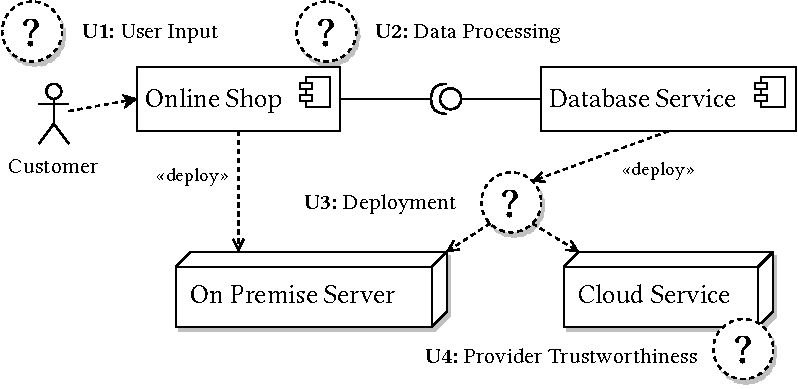
\includegraphics[width=0.9\textwidth]{figures/chapter3/onlineshop-architecture.pdf}
    \caption[Combined component and deployment diagram of the running example.]{Combined component and deployment diagram showing the software architecture of the online shop running example with annotated uncertainty sources depicted as circled question marks.}
    \label{fig:runningexample:architecture}
\end{figure}

The software architecture is depicted in \autoref{fig:runningexample:architecture}.
It consists of two components and two deployment locations. 
The \emph{Online Shop} component serves as the interface for customers while the \emph{Database Service} is used to persist information about customers, purchases, and the shop's inventory.
Both components are connected through an interface which is provided by the \emph{Database Service}.
The \emph{Online Shop} component is deployed on an \emph{On Premise Server} while the \emph{Database Service} can either be deployed locally on the same server or alternatively on a \emph{Cloud Service} for better scalability.

Customers interact directly with the \emph{Online Shop} component.
The running example comprises three usage scenarios.
First, customers input search details and request to view available items.
Second, they select an item to purchase and enter payment and shipping details.
In both scenarios, the input is processed in the \emph{Online Shop} component first.
Afterward, data is exchanged with the database, e.g., to query the inventory, or to store the purchase history.
The third usage scenario considers users that request static information like support contact addresses.
This information is provided directly by the \emph{Online Shop} component without any communication with the database.

We consider two types of data in the running example: The online shop's public information, and the user's private purchase details.
The former is publicly available and does not have to be protected---on the contrary, the online shop benefits from the public availability of this information.
The latter can be classified as personal or sensitive information for which confidentiality requirements apply.
Public availability of the customers' shopping and payment details would harm their privacy and might cause fraud or theft.
The European \acf{GDPR} demands that personal data of European citizens is only allowed to be stored and processed on European servers or on servers which ensure \enquote{an adequate level of protection} \cite[Art.~45]{council_of_european_union_regulation_2016}.
In the following, we assume that the online shop is operated in Europe, which implies that data processing on the \emph{On Premise Server} complies with this confidentiality requirement.
Depending on the cloud's server location and the trustworthiness of the provider, the storage on the \emph{Cloud Service} might violate this requirement.
Additional confidentiality requirements can include the user input, which has to be neither erroneous nor malicious, and also has to be validated and encrypted as part of the \emph{Online Shop} processing.

\begin{figure}
    \centering
    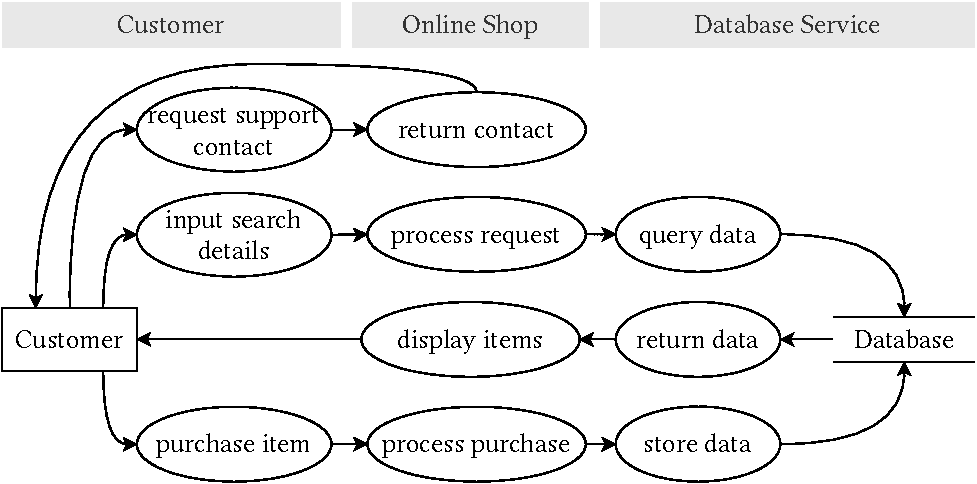
\includegraphics[width=0.9\textwidth]{figures/chapter3/onlineshop-dfd.pdf}
    \caption[Exemplary \acf*{DFD} of the running example.]{Exemplary \acf*{DFD} illustrating possible data flows through the online shop running example. The gray boxes indicate the user and components of the software architecture.}
    \label{fig:runningexample:dfd}
\end{figure}

We illustrate the behavior and data flows of the running example as \acf{DFD} in \autoref{fig:runningexample:dfd}.
In addition to the \ac{DFD} elements introduced in \autoref{sec:foundations:dfd}, we depict the users and components using gray boxes \cite{seifermann_architectural_2022}.
The upper half of the diagram represents the flow of query requests from the user via the online shop to the database and the response containing available items from the database to the user.
Additionally, it shows the request for support information.
In our simplified example, both data flows do not contain sensitive information.
Thus, no confidentiality requirements apply.
In the lower half, the customer purchases an item.
The purchase is processed on the online shop and then stored in the database.
This data flow is subject to confidentiality requirements.





\section{Exemplary Uncertainty Sources}%
\label{sec:runningexample:uncertainty}

As described previously in \autoref{sec:foundations:uncertainty}, uncertainty sources can exist within the software system and its environment \cite{acosta_uncertainty_2022}.
In \autoref{fig:runningexample:architecture} and in the following, we represent uncertainty sources in diagrams as circled question marks.
We introduce four exemplary yet common sources of uncertainty to our running example:

\begin{enumerate}[label=\textbf{U\arabic*}]
    \item The users' input is a source of uncertainty. Although certain behavior regarding entered information can be expected already at design time, it cannot be guaranteed. % https://arc3n.abunai.dev/uncertainty/52 (Connector)
    \item The data processing is still uncertain. This can be the case due to an open design decision or due to the black box nature of a third-party off-the-shelf component. % https://arc3n.abunai.dev/uncertainty/35 (Behavior)
    \item The component deployment is an uncertainty source. This can be caused by missing design decisions or dynamic reconfiguration at runtime, e.g., due to load balancing. % https://arc3n.abunai.dev/uncertainty/59 (Component)
    \item The trustworthiness of a resource provider, which is used as a deployment location for a component or service, is uncertain and can only be assured, e.g., with policies. % https://arc3n.abunai.dev/uncertainty/48 (External)
\end{enumerate}

We annotate the first Uncertainty \U{1} to the customer using the online shop.
Humans are a common uncertainty source within the literature, often referred to as \emph{human in the loop} \cite{perez-palacin_uncertainties_2014,ramirez_taxonomy_2012}.
Although the user input is uncertain, we can assume different input classes, e.g., valid input as expected, erroneous input due to human failure, or malicious input.

The second uncertainty source \U{2} considering the data processing is annotated to the \emph{Online Shop} component and its connection to the \emph{Database Service}.
This could be uncertain due to the black-box principle of software components \cite{reussner_modeling_2016} or due to a yet-to-be-defined design decision \cite{lytra_supporting_2013}.
In our example, this could affect confidentiality if we do not know whether all requests to the \emph{Database Service} are encrypted before sending.
Additionally, input validation could be part of the processing, which analyzes the users' input to counter Uncertainty \U{1}.
Also, combinations of input validation and encryption are imaginable.

The third uncertainty source \U{3} affects the deployment of the \emph{Database Service} and is annotated on the associated arrow.
Deployment decisions could be still uncertain at design time \cite{mcconnell_software_1998}, or depend on the runtime situation, e.g., in the context of \acfp{SAS} \cite{weyns_introduction_2020}.
In \autoref{fig:runningexample:architecture}, we show two possible deployment locations, with the \emph{Database Service} being either deployed on-premise or in the cloud.

The fourth uncertainty source \U{4} is annotated to the \emph{Cloud Service} and questions the providers' trustworthiness.
Providers could void confidentiality either intentionally, e.g., by misusing data \cite{costante_privacy-aware_2013}, or unintentionally, e.g., due to the lack of proper security requirements and appropriate measures \cite{firesmith_specifying_2004}.
To that end, we can only assume the trustworthiness and categorize whether providers are trustworthy enough or not.

Other and additional uncertainty sources are also possible within the running example, see \arcen.
We selected these uncertainties as they demonstrate different locations, types, and origins, while still keeping the running example simple and easy to understand.





\section{Summary and Outlook}%
\label{sec:runningexample:summary}

In this chapter, we introduced a running example that will be used throughout this thesis.
Already a software system of the size of our running example shows the challenge of dealing with multiple uncertainty sources.
Uncertainty sources and impact locations arise at different points within the software system and its environment, which might cause complex interrelations and interactions \cite{camara_uncertainty_2024} regarding confidentiality.
Especially in larger software systems, analyzing them manually is not expedient.
Thus, we need proper modeling, analysis, and mitigation strategies to ensure confidentiality.

Note, that the \ac{DFD} shown in \autoref{fig:runningexample:dfd} also depends on the outcome of the uncertainty sources \U{1} -- \U{4}.
Uncertainty \U{1} could alter the customer process \emph{input search details}, or Uncertainty \U{3} could affect the structure of the \ac{DFD}.
Additionally, the concrete form of the \ac{DFD} depends on the level of abstraction \cite{demarco_structure_1979}.
Building on previous advances in uncertainty representation \cite{garlan_software_2010,troya_uncertainty_2021}, we find that:

\finding{Even small software systems like our running example can have many corresponding data flow diagrams under uncertainty. 
Uncertainty hinders precise modeling and analysis when not included properly within the model.}

The presentation of the running example was based on \acp{DFD} and uncertainty which both have been introduced in \readingpath{ch:foundations}.
Next, we use the running example to give an overview of all contributions in \readingpath{ch:overview}.
We modeled the software architecture of the running example based on the \acf{PCM}.
The model files can be found in our data set \cite{dataset}.
An overview and first impression is given in \autoref{sec:appendix:runningexample}.





\section{In Simpler Words}%
\label{sec:runningexample:simple}

A simple running example makes it easier to understand complex ideas.
We introduce the running example of an online shop known from everyday life.
Online shops deal with customer data and are thus required to protect that data and keep it confidential.
Additionally, we presented different sources of uncertainty in our example.
Examples are the behavior of customers or the trustworthiness of cloud service providers.
Even in this simple example, we can see how this uncertainty harms confidentiality.
For example, if we are unsure whether providers behave maliciously, customers' stored data could be threatened.
One approach to face the challenge of analyzing confidentiality under uncertainty will be presented in the remainder of this thesis.